% E.2 △ABC 等腰 AB=AC=10, BC=12. 高 AH=8. D 在 BA 上(BD=t), E 在 CB 上(CE=2t)
% B(-6,0), C(6,0), A(0,8). 示例 t=3: D 在 BA 上, BD=3 → D = B + 3/10·(A-B) = (-6,0)+0.3·(6,8) = (-4.2, 2.4)
% E 在 CB 上, CE=6 → E = C + 6/12·(B-C) = (0,0)
\documentclass[tikz,border=4pt]{standalone}
\usepackage{ctex}
\usepackage{amsmath}
\usetikzlibrary{calc}
\begin{document}
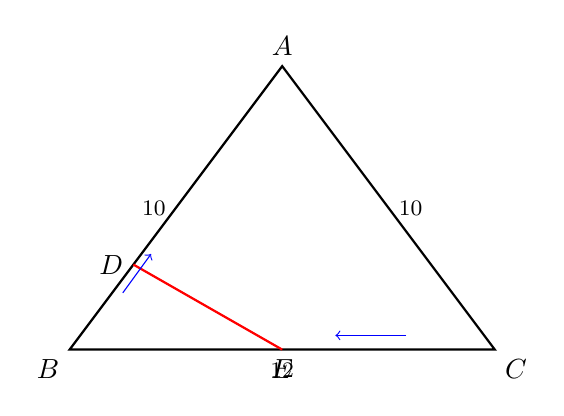
\begin{tikzpicture}[scale=0.45, thick]
  \coordinate (B) at (-6,0);
  \coordinate (C) at (6,0);
  \coordinate (A) at (0,8);
  \coordinate (D) at (-4.2, 2.4);
  \coordinate (E) at (0,0);

  \draw (A)--(B)--(C)--cycle;
  \draw[red, thick] (D)--(E);

  \draw[->, blue, thin] (-4.5,1.6) -- (-3.7,2.7);
  \draw[->, blue, thin] (3.5,0.4) -- (1.5,0.4);

  \node[above] at (A) {$A$};
  \node[below left] at (B) {$B$};
  \node[below right] at (C) {$C$};
  \node[left] at (D) {$D$};
  \node[below] at (E) {$E$};

  \node[left, font=\footnotesize] at ($(A)!0.5!(B)$) {$10$};
  \node[right, font=\footnotesize] at ($(A)!0.5!(C)$) {$10$};
  \node[below, font=\footnotesize] at ($(B)!0.5!(C)+(0,-0.1)$) {$12$};
\end{tikzpicture}
\end{document}
